\setlength{\columnsep}{3pt}
\begin{flushleft}

There are 2 types of process:

\begin{figure}[h!]
	\centering
	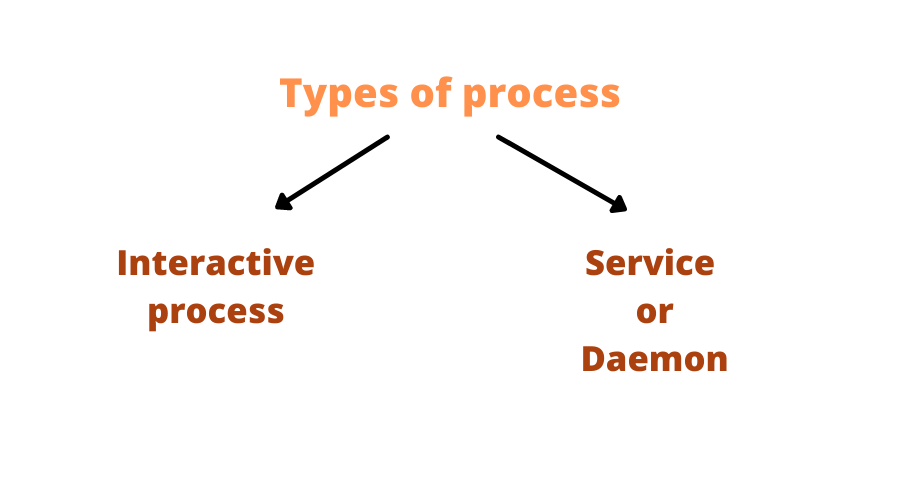
\includegraphics[scale=.55]{content/chapter12/images/newp.png}
\end{figure}

Let's see each of these in detail.
\newpage

\begin{enumerate}
	\item \textbf{Interactive process}
	\begin{itemize}
		\item Interactive process are invoked by a user and can interact with the user.
		\item Classified into two types:
		
		\begin{figure}[h!]
			\centering
			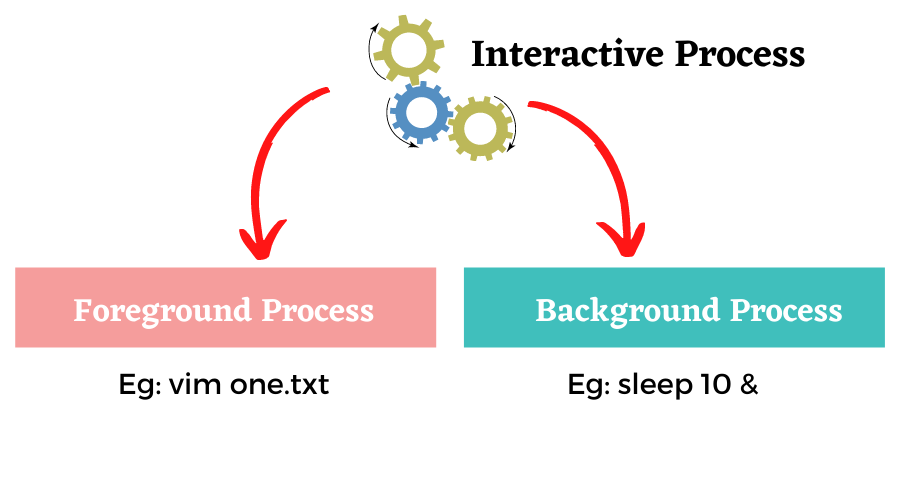
\includegraphics[scale=.45]{content/chapter12/images/interactive.png}
			\caption{Types of interactive process}
			\label{fig:type}
		\end{figure}
		
		\begin{enumerate}
			\item \textbf{Foreground process}: Process that you are currently interacting with using the terminal.
			\item \textbf{Background process}: 
			\begin{itemize}
				\item These process do not interact with the user \& they run in the background.
				\item To run process in background, use \textbf{"\&"} by appending it at the end of command.
				\bigskip
				\begin{tcolorbox}[breakable,notitle,boxrule=-0pt,colback=pink,colframe=pink]
					\color{black}
					\fontdimen2\font=9pt
					Syntax: command \&
					\fontdimen2\font=4pt
				\end{tcolorbox}
				Eg: Run \textbf{sleep} command in background:
				\begin{tcolorbox}[breakable,notitle,boxrule=-0pt,colback=black,colframe=black]
					\color{green}
					\fontdimen2\font=9pt
					\#  sleep 60 \&
					\fontdimen2\font=4pt
				\end{tcolorbox}
			\end{itemize}
		\end{enumerate}
		
		\newpage
		
		
		
		\item \textbf{Commands for interactive process}
		\begin{enumerate}
			\item \textbf{jobs}: To check all interactive process.
			\bigskip
			\begin{tcolorbox}[breakable,notitle,boxrule=-0pt,colback=pink,colframe=pink]
				\color{black}
				\fontdimen2\font=9pt
				Syntax: jobs
				\fontdimen2\font=4pt
			\end{tcolorbox}
			
			Eg: If there are any interactive process, \textbf{jobs} will list all process:
			\begin{tcolorbox}[breakable,notitle,boxrule=-0pt,colback=black,colframe=black]
				\color{green}
				\fontdimen2\font=9pt
				\#  jobs
				\color{white}
				\newline
				[1]+  Stopped                 vim one.txt
				\newline
				[2]-  Running                 sleep 10 \&
				\fontdimen2\font=4pt
			\end{tcolorbox}
			Explaination of output:
			\begin{itemize}
				\item \textbf{[1],[2]}: Interactive process ids.
				\item \textbf{"+"}: Job used as default for the fg or bg utilities. 
				\item \textbf{"-"}: Default job if the current default job were to exit.
			\end{itemize}	
			
			\bigskip
			
			\item \textbf{bg}: To change the state of a background process from \textbf{"Stopped"} to \textbf{"Running"}.
			\begin{tcolorbox}[breakable,notitle,boxrule=-0pt,colback=pink,colframe=pink]
				\color{black}
				\fontdimen2\font=9pt
				Syntax: bg \%[job\_id]
				\fontdimen2\font=4pt
			\end{tcolorbox}
			
			Eg: Execute \textbf{sleep} command as shown and press \textbf{CTRL+Z} to push the process in background in \textbf{"Stopped"} state.
			\begin{tcolorbox}[breakable,notitle,boxrule=-0pt,colback=black,colframe=black]
				\color{green}
				\fontdimen2\font=9pt
				\# sleep 300 
				\color{yellow}
				\newline
				Press CTRL+Z
				\fontdimen2\font=4pt
			\end{tcolorbox}
			Next, execute jobs command to confirm shown output:
			\begin{tcolorbox}[breakable,notitle,boxrule=-0pt,colback=black,colframe=black]
				\color{green}
				\fontdimen2\font=9pt
				\# jobs 
				\color{white}
				\newline
				[1]+  Stopped                 sleep 300
				\fontdimen2\font=4pt
			\end{tcolorbox}
			Execute \textbf{bg} command to change the state of the command to \textbf{"Running"}.
			\begin{tcolorbox}[breakable,notitle,boxrule=-0pt,colback=black,colframe=black]
				\color{green}
				\fontdimen2\font=9pt
				\# bg \%1
				\color{white}
				\newline
				[1]+ sleep 300 \&
				\newline
				\color{green}
				\# jobs
				\color{white}
				\newline
				\color{white}
				[1]+  Running             sleep 300 \&
				\fontdimen2\font=4pt
			\end{tcolorbox}
			
			\bigskip
			\bigskip
			
				\item \textbf{fg}: To run the background process in foreground.
			\begin{tcolorbox}[breakable,notitle,boxrule=-0pt,colback=pink,colframe=pink]
				\color{black}
				\fontdimen2\font=9pt
				Syntax: fg \%[job\_id]
				\fontdimen2\font=4pt
			\end{tcolorbox}
			
			Eg: Execute \textbf{sleep} command in background as shown:
			\begin{tcolorbox}[breakable,notitle,boxrule=-0pt,colback=black,colframe=black]
				\color{green}
				\fontdimen2\font=9pt
				\# sleep 300 \&
				\fontdimen2\font=4pt
			\end{tcolorbox}
			Next, execute jobs command to confirm shown output:
			\begin{tcolorbox}[breakable,notitle,boxrule=-0pt,colback=black,colframe=black]
				\color{green}
				\fontdimen2\font=9pt
				\# jobs 
				\color{white}
				\newline
				[1]+  Running                 sleep 300 \&
				\fontdimen2\font=4pt
			\end{tcolorbox}
			Execute \textbf{fg} command to bring \textbf{sleep} command in foreground.
			\begin{tcolorbox}[breakable,notitle,boxrule=-0pt,colback=black,colframe=black]
				\color{green}
				\fontdimen2\font=9pt
				\# fg \%1
				\color{white}
				\newline
				[1]+ sleep 300 \&
				\newline
				\color{green}
				\# jobs
				\color{white}
				\newline
				[1]+  Running                 sleep 300 \&
				\fontdimen2\font=4pt
			\end{tcolorbox}
			
		\end{enumerate}
		

	
	\end{itemize}
\newpage
	\item \textbf{Daemon}
	\begin{itemize}
		\item Daemon are process that are running in background on the computer.
		\item They provide some services, but they do not interact with the console.
		\item \textbf{Server software are implemented as a daemon.}
		\item Eg: httpd, sshd, nfs etc.
		\item Command to check daemon status:
		\bigskip
		\begin{tcolorbox}[breakable,notitle,boxrule=-0pt,colback=pink,colframe=pink]
			\color{black}
			\fontdimen2\font=9pt
			Syntax: systemctl status daemon\_name
			\fontdimen2\font=4pt
		\end{tcolorbox}
		Eg:
		\begin{figure}[h!]
			\centering
			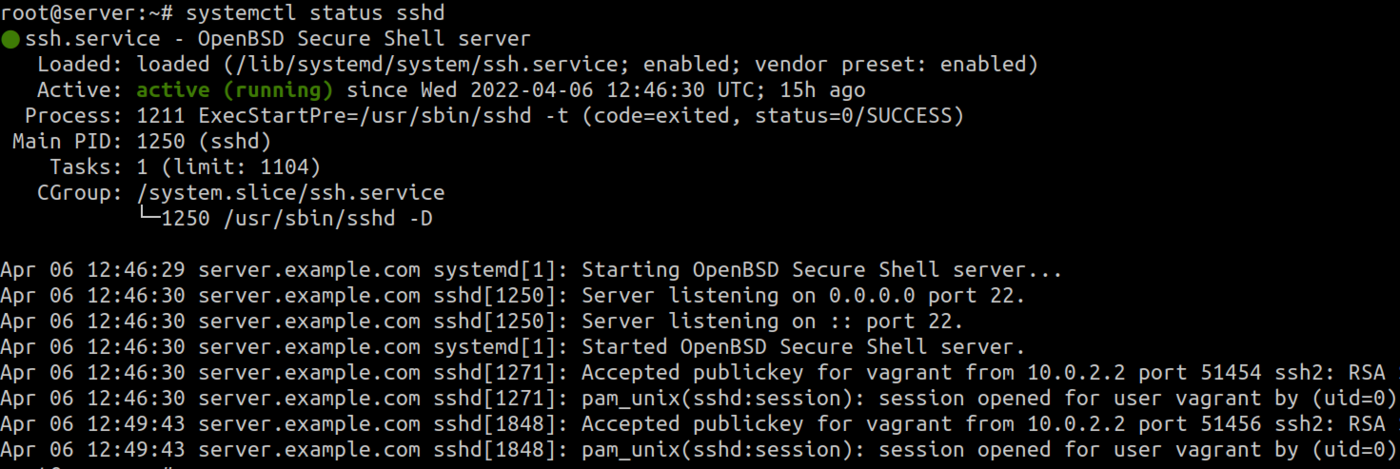
\includegraphics[scale=.25]{content/chapter12/images/proc.png}
			\caption{Sample output}
			\label{fig:process23}
		\end{figure}
	\end{itemize}
	
	

	
	
\end{enumerate}
	
		
\end{flushleft}

\newpage


